\section{Appendix: Impeller Angle}
\label{sec:impeller_angle}
This section will discuss the estimation of the impeller angle. The impeller angle was estimated using a digital protractor. 

\begin{figure}[h]
    \centering
    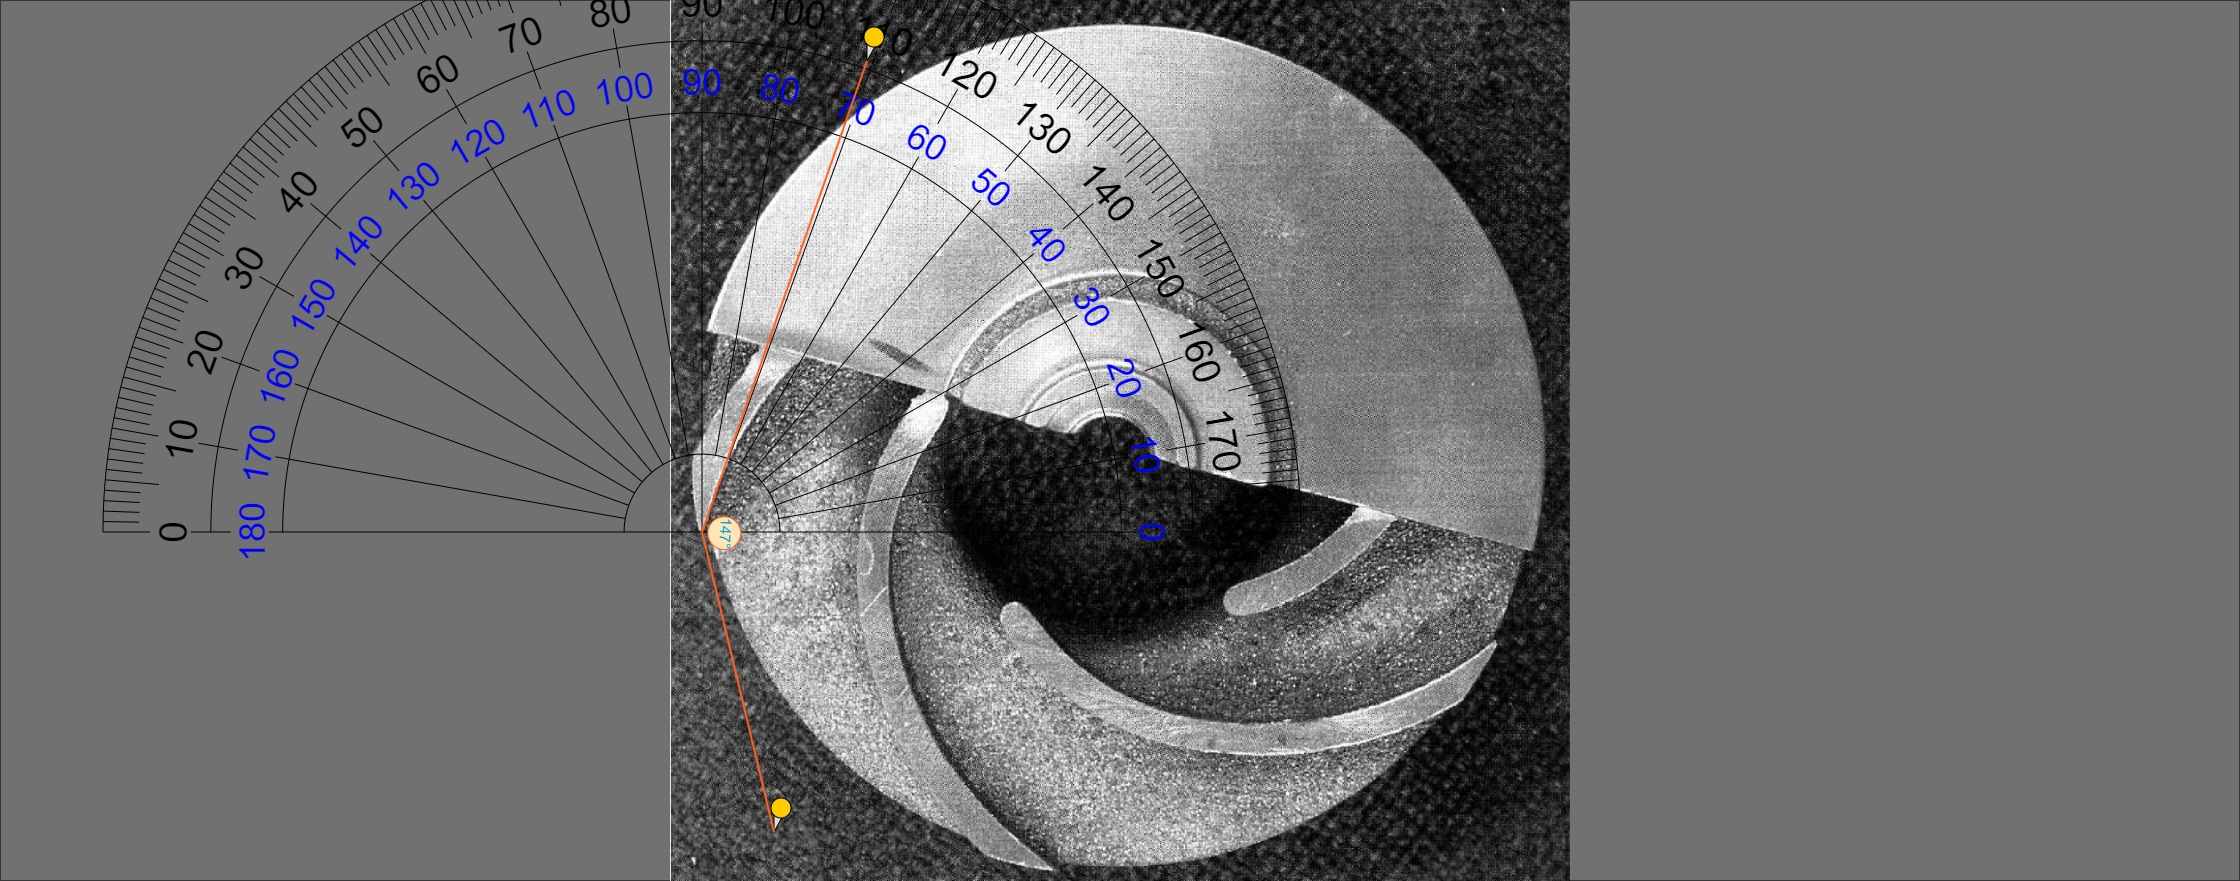
\includegraphics[width=0.7\textwidth]{Sections/Figures/Impeller Angle.jpg}
    \caption{Estimation of the impeller angle using digital protractor}
    \label{fig:impeller_angle}
\end{figure}
The impeller angle was estimated using a digital protractor, as shown in Figure \ref{fig:impeller_angle}. The impeller angle was measured to be 
\begin{align*}
    \beta_2 &= 180^\circ - 147^\circ = 33^\circ
\end{align*}
From equation (\ref{ideal_turbo_machinary}), the ideal operating curve is
\begin{align*}
    \Psi &= 1 - \Phi \cot{\beta_2} \\
    &= 1 - \Phi \cot{33^\circ} \\
    &= 1 - 1.540 \Phi
\end{align*}